\chapter{Bonds}
\label{bonds}

A bond is an instrument that represents a loan made by an investor to a borrower (typically corporate or governmental). Bonds are used by companies, municipalities, states, and sovereign governments to finance projects and operations. 

Owners of bonds are debt-holders, or creditors of the issuer. Bond details include the principal (the loan amount), the end date (when the loan principal is due to be paid to the bond owner) and usually includes the terms for variable or fixed interest payments made by the borrower.

The \emph{coupon} is the interest rate that the issuer pays to the holder. This rate can be fixed throughout the life of the bond but it can also vary with a money market index, such as LIBOR, or it can be even more exotic.

\section{Valuing a Bond}
\label{sec:bond_pricing}

The value of a bond can be computed as the present discounted value of future cash flows generated by the bond itself.

For example consider a 3-years bond with a face value of \euro{100} providing coupons at a 6\% rate annually. Assume also that the discount rates are 5.0\% 5.8\% and 6.4\% for 1, 2, 3 years. The value will be then:

\begin{equation*}
P_{\mathrm{bond}}=6e^{-0.05\cdot 1}+6e^{-0.058\cdot 2}+106e^{-0.064\cdot 3}
\end{equation*}

\begin{ipython}
from math import exp

rates = {1:0.05, 2:0.058, 3:0.064}
N = 100
maturity = 3
fixed_coupon = 0.06
price = 0

for tau in range(1, maturity+1):
    price += N * fixed_coupon * exp(-rates[tau] * (tau))
price += N * exp(-rates[tau] * (tau))

print ("{:.2f} EUR".format(price))
\end{ipython}
\begin{ioutput}
98.53 EUR
\end{ioutput}

\subsection{Yield to Maturity}
The \emph{yield to maturity} is the interest rate that makes the present value of the future coupon payments equal to the current bond price, that is, for a known price $P_0$, the yield is the solution $y$ to the equation

\begin{equation}
P = \sum_{t=1}^T e^{-yt}C + e^{-yT}N 
\label{eq:yield_to_maturity}
\end{equation}
where $C$ is the coupon end $N$ the nominal.

Finding the yield to maturity is equivalent to find the zeros of Eq.~\ref{eq:yield_to_maturity}.
To find the zeros of a function $f(x)$ means to determine the values $\hat{x}$ such that $f(\hat{x})=0$ and the process is equivalently called finding the roots of $f(x)$. There are various methods to achieve that, in the following we will see two of them.
\label{sec:root_finding}
\emph{Bisection}~\cite{bib:bisection} method is considered the simplest one-dimensional root-finding algorithm.
Suppose we know two points of an interval $[a,b]$, and that $f (a)< 0$ and $f(b)> 0$.
Since the value of $f(a)$ is negative and $f(b)$ is positive, the bisection method assumes that the root $x$ lies somewhere between $a$ and $b$.

Taking the midpoint of this $[a, b]$ interval as $c$, the bisection method then evaluates this value as $f(c)$.
If $f(c) = 0$ or is very close to zero by some predetermined error tolerance value, then a root is declared as found. If $f(c)< 0$, then we may conclude that a root exists along the interval $[c, b]$, or along the interval $[a,c]$ otherwise.

On the next evaluation, $c$ is replaced as either $a$ or $b$ accordingly. With the new interval shortened, the bisection method repeats with the same evaluation to determine the next value of $c$. This process continues, shrinking the width of the interval until the root is determined as found. Figure~\ref{fig:bisection} shows an example of bisection algorithm application.

\begin{figure}[htbp]
\centering
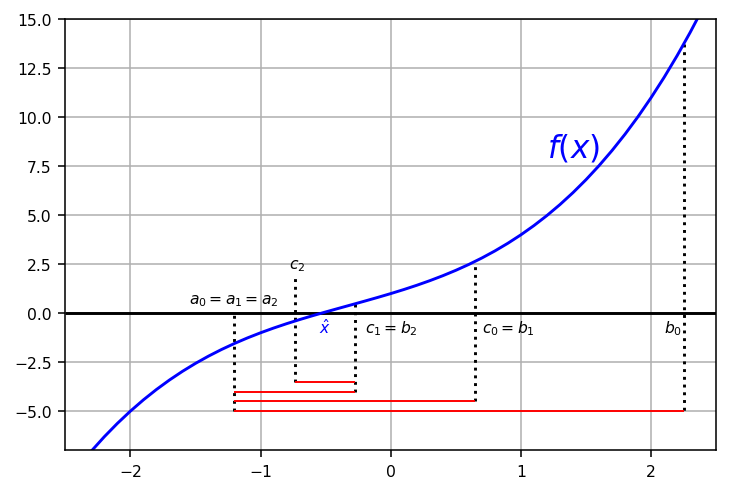
\includegraphics[width=0.7\linewidth]{figures/bisection}
\caption{Example of bisection algorithm to find the roots of a function $f(x)$.}
\label{fig:bisection}
\end{figure}

The biggest advantage of the bisection method is it is guaranteed to converge to an approximation of the root, given a predetermined error tolerance level and the maximum number of iterations allowed. It should be noted that the bisection method does not require knowledge of the derivative of the unknown function. In certain continuous functions, the derivative could be complex or even impossible to calculate. This makes this method extremely valuable for working on functions that are not smooth.
Contrary, its major drawback is that it takes up more computational time in the iterative evaluation as compared to other root-finder methods. 

Although this method is simple enough to be quickly implemented in \texttt{python} we will opt for the surely bug free version available in \texttt{scipy.optimize.bisect} (for the usage of \texttt{args} see Section~\ref{sec:kwargs_args}).

\begin{ipython}
from scipy.optimize import bisect 

def ytom(y, N, C, P0, maturity_years, tenor=1): 
	price = 0
	for p in range(1, int((maturity_years/tenor)+1)):
		price += C*tenor*N/(1+y*tenor)**p
	price += N/(1+y*tenor)**p - P0 
	return price

print (bisect(ytom, -0.3, 1, args=(100, 0.05, 95, 6, 0.5)))
\end{ipython}
\begin{ioutput}
0.060047636994841024
\end{ioutput}

An alternative algorithm is the \emph{Brent's method}~\cite{bib:brent} which combines the advantages of both bisection and secant (another root-finding algorithm) methods. Its \texttt{python} implementation is in \texttt{scipy.optimize.brentq}.

\begin{ipython}
from scipy.optimize import brentq
    
print (brentq(ytom, -0.3, 1, args=(100, 0.05, 95, 6, 0.5)))
\end{ipython}
\begin{ioutput}
0.06004763699594817
\end{ioutput}

\noindent
The results match down to the eleventh digit.

\subsection{Duration}
The duration of a bond is the \emph{weighted average maturity} of the bond

\begin{equation}
\textrm{duration} = \sum_{i=1}^{n} t_i \left[\cfrac{C_i D_i}{P}\right] 
\end{equation}
where $C_i$ is the cash flow in period $t_i$, $D_i$ is the corresponding discount factor and $P$ is the bond price.
Knowing the bond yield from Eq.~\ref{eq:yield_to_maturity} the previous equation becomes:
\begin{equation}
\textrm{duration} = \sum_{i=1}^{n} t_i \left[\cfrac{C_i e^{-yt_i}}{P}\right] 
\label{eq:duration}
\end{equation}

This quantity is sometimes referred to as \emph{Macaulay Duration}. By accounting for the present value of future bond payments, the Macaulay duration helps an investor to evaluate and compare bonds independent of their time to maturity.
It estimates how many years it will take for an investor to be repaid the bond’s price by its total cash flows.

Imagine a three-year bond with a face value of \$100 that pays a 10\% coupon semi-annually and has a yield to maturity (YTM) of 6\%. We will first compute the present value of the bond and then calculate its Macaulay duration.

\begin{ipython}
def bond_pv(N, C, r, maturity, tenor=1):
	price = 0
	for tau in range(1, int((maturity/tenor)+1)):
		price += N * C*tenor / (1+r*tenor)**(tau)
	price += N / (1+r*tenor)**(tau)
	return price

def mac_duration(N, C, y, maturity, P0, tenor=1): 
	d=0
	for tau in range(1, int((maturity/tenor)+1)):
		d += tau*N*C*tenor/(1+y*tenor)**tau/P0
	d += tau*N/(1+y*tenor)**tau/P0 
	return d

P0 = bond_pv(100, 0.1, 0.06, 3, 0.5)
print ("Bond price: {:.2f}".format(P0))

dur = (mac_duration(100, 0.1, 0.06, 3, P0, 0.5))
print ("Duration: {:.2f}".format(dur))
\end{ipython}
\begin{ioutput}
Bond price: 110.83
Duration: 5.37
\end{ioutput}

This result can be interpreted by saying that it will take about two years and 7 months to be repaid for the bond expenses.

Equation~\ref{eq:duration} connects the bond price to the yield through duration. When a small change in yield $\Delta y$ happens
\begin{equation}
\Delta P = \cfrac{dP}{dy}\Delta y
\label{eq:price_1st_order}
\end{equation}
\noindent
Computing the derivative of the bond price from Eq.~\ref{eq:yield_to_maturity} we get

\begin{equation}
\Delta P = -\Delta y\sum_i C_i t_i e^{-yt_i}
\label{eq:price_yield}
\end{equation}
\noindent
which indicates there is a negative relationship between $P$ and $y$ (i.e. when bond yield increases the bond price decrease). 

Substituting Eq.~\ref{eq:duration} into Eq.~\ref{eq:price_yield} 
\begin{equation}
\Delta P = -PD\Delta y \quad\rightarrow\quad \cfrac{\Delta P}{P} = -D\Delta y
\label{eq:price_sens}
\end{equation}

This is an approximate relationship between percentage changes in a bond price and changes in its yield.

Consider a 3-year 10\% coupon bond with a face value of 100\$. Suppouse its yield is 12\% and that coupon payments of 5\$ are made every 6 months. Using the previous functions it is possible to compute bond price and duration

\begin{ipython}
price = bond_pv(100, 0.1, 0.12, 3, 0.5)
print ("Price: {:.3f}".format(price))

dur = mac_duration(100, 0.1, 0.12, 3, price, 0.5)
print ("Duration: {:.3f}".format(dur))
\end{ipython}
\begin{ioutput}
Price: 95.083
Duration: 5.310
\end{ioutput}

Replacing those values into Eq.~\ref{eq:price_sens} it is possible to estimate the sensitivity of the bond price to small changes of the yield.
Assuming for example an yield variation of 10 basis points
\begin{ipython}
dP = -price*dur*0.001
print ("DeltaP: {:.3f}".format(dP))
print ("P+DP: {:.3f}".format(price+dP))
\end{ipython}
\begin{ioutput}
DeltaP: -0.505
P+DP: 94.578
\end{ioutput}

To check how good is this approximation we can compute the bond price assuming the new yield
\begin{ipython}
today = date.today()

price = bond_pv(100, 0.1, 0.121, 3, 0.5)
print ("Price: {:.3f}".format(price))
\end{ipython}
\begin{ioutput}
Price: 94.845
\end{ioutput}

Which is in good agreement with the approximate calculation.
When the yield variation is larger the simple linear approximation is not valid anymore as shown in Fig.~\ref{fig:bond_sensitivity}.

\begin{figure}[htbp]
\centering
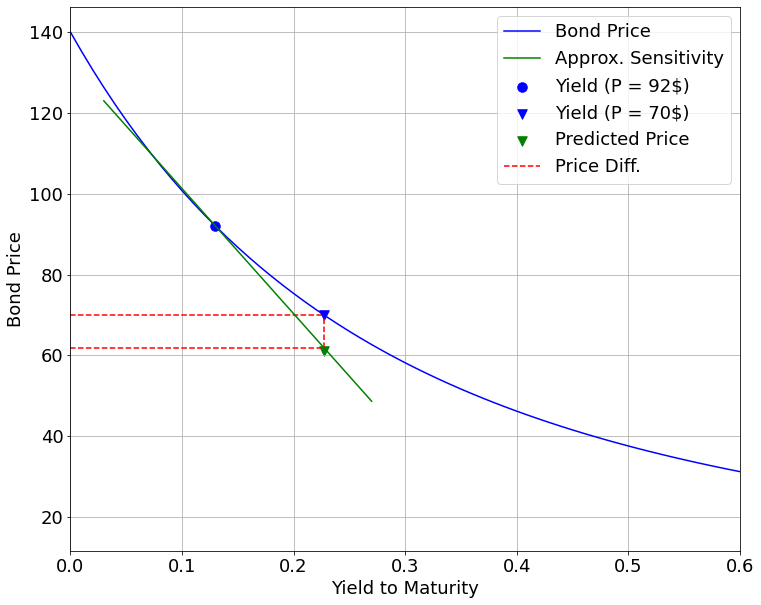
\includegraphics[width=0.7\linewidth]{figures/bond_duration}
\caption{Bond price sensitivity to yield variation. For large movements of the yield the simple linear approximation given by
 Eq.~\ref{eq:price_sens} is not valid anymore.}
\label{fig:bond_sensitivity}
\end{figure}

\subsection{Price Value of a Basis Point}
A very common risk measure is the sensitivity of the price of a bond to changes in its yield. The price value of a basis point, PVBP, sometimes called the dollar value of a basis point, or $DV01$, measures the decline in price associated with a one basis point increase in the yield.

\begin{equation}
DV01 = −\cfrac{dP}{dy}\times 0.0001
\end{equation}

$DV01$ can be computed directly, by computing the price at the current yield, adding one basis point to the yield, and recomputing the price.

$DV01$ can also be computed directly from duration. In particular, we have seen that $dP/P = -D dy$. Hence $dP = -D Pdy$ and

\begin{equation}
DV01 = -D P \times 0.0001
\end{equation}

\subsubsection{Modified Duration}
In the previous analysis we have assumed continuous compounding. If instead $y$ is expressed with a compounding frequency of $m$ times per year then 
\begin{equation}
\Delta P = \cfrac{PD\Delta y}{1+y/m}
\end{equation}
\noindent
The quantity $D^{*}$, defined by
\begin{equation}
D^{*} = \cfrac{D}{1+y/m}
\end{equation}
\noindent
is referred to as \emph{modified duration}. 

\subsection{Convexity}
The duration relationship studied in the previous Section is valid only for small changes in yields. Since Eq.~\ref{eq:price_1st_order} is just a Taylor expansion to first order, to improve its accuracy we need to go to higher orders

\begin{equation}
\Delta P = \cfrac{dP}{dy}\Delta y + \cfrac{1}{2} \cfrac{d^2 P}{dy^2}\Delta y^2 = -D\Delta y + \cfrac{1}{2} \textrm{Conv} \Delta y^2 
\end{equation}
\noindent
The quantity $\textrm{Conv} = \frac{\sum_i C_i t_i^2 e^{-yt_i}}{P}$ is called \emph{convexity} and parametrizes the behaviour of the bond price for large yield variations.

Considering a portfolio of bonds, the convexity tends to be greatest when it provides payments evenly over a long period of time. Contrary it is least when the payments are concentrated around on particular point in time. 

Choosing a portfolio of assets with net duration and net convexity both close to zero, we make ourselves immune to relatively large shifts in the zero curve (i.e. large movements of the yield)

\subsection{Duration, Convecxity and DV01 of a Bond Portfolio}
The duration of a bond portfolio, $D_p$, is computed as the weighted average of the durations of the individual
bonds:
\begin{equation}
D_p = \sum_{i=1}^{K} \alpha_i D_i
\end{equation}
where $K$ is the number of different bonds and $\alpha_i$ is the fraction of portfolio dollars invested in bond $i$. Similarly, the convexity of a bond portfolio, Conv$_p$, is the weighted average of the convexities of the individual bonds.
\begin{equation}
\textrm{Conv}_p = \sum^{K}_{i=1} \alpha_i \textrm{Conv}_i
\end{equation}
The $DV01_p$ of a portfolio is defined as the change in value resulting from equal one basis point declines in all yields. Let $DV01_i$ represent the dollar value of a basis point associated with the i$^{th}$ bond. Then
\begin{equation}
DV01_p = \sum^{K}_{i=1}x_i DV01_i
\end{equation}
where $x_i$ is the number of bonds of type $i$ in the portfolio.

\section*{Exercises}
\begin{question}
A Treasury bond has a coupon of 9\%, a face value of 1000 USD and matures 10 years from today. For a treasury bond the interest on the bond is paid in semi-annual coupons. The current risk-less interest rate is 12\% (compounded semi-annually).
\begin{enumerate}
\item Suppose you purchase the Treasury bond described above and immediately thereafter the risk-less interest rate falls to 8\%. (compounded semi-annually). What would be the new market price of the bond?
\item What is your best estimate of what the price would be if the risk-less interest rate was 9\% (compounded semi-annually) ?
\end{enumerate}
\end{question}

\cprotEnv\begin{solution}
\begin{ipython}
import numpy as np

N = 1000
maturity = 10
coupon = 0.09
tenor = 0.5
rates = {i:0.08 for i in range(1, int((maturity/tenor)+1))}

price = 0
for tau in range(1, int((maturity/tenor)+1)):
    price += N * coupon*tenor / (1+rates[tau]*tenor)**(tau)
price += N / (1+rates[tau]*tenor)**(tau) 

print (f"{price:.2f} USD")
\end{ipython}
\begin{ioutput}
1067.95 USD
\end{ioutput}

\begin{ipython}
rates = {i:0.09 for i in range(1, int((maturity/tenor)+1))}
	
price = 0
for tau in range(1, int((maturity/tenor)+1)):
    price += N * coupon*tenor / (1+rates[tau]*tenor)**(tau)
price += N / (1+rates[tau]*tenor)**(tau) 
	
print (f"{price:.2f} USD")
\end{ipython}
\begin{ioutput}
1000.00 USD
\end{ioutput}
\end{solution}

\begin{question}
A 100 USD, 10 year bond was issued 7 years ago at a 10\% annual interest rate. The current interest rate is 9\%.The current price of the bond is 100.917 USD. Use annual, discrete compounding. Calculate the bonds yield to maturity.
\end{question}

\cprotEnv\begin{solution}
\begin{ipython}
from scipy.optimize import brentq

def ytom(y, N, C, P0, maturity_years, tenor=1): 
    price = 0
    for p in range(1, int((maturity_years/tenor)+1)):
        price += C*tenor*N/(1+y*tenor)**p
    price += N/(1+y*tenor)**p - P0 
    return price

y = brentq(ytom, -0.3, 1, args=(100, 0.10, 100.917, 3, 1))
print (f"yield to maturity: {y:3f}")
\end{ipython}
\begin{ioutput}
yield to maturity: 0.096
\end{ioutput}    
\end{solution}

\begin{question}
Suppose you are trying to determine the interest rate sensitivity of two bonds. Bond 1 is a 12\% coupon bond with a 7-year maturity and a 1000 USD principal. Bond 2 is a ‘zero-coupon’ bond that pays 1120 USD after 7 year.The current interest rate is 12\%.
\begin{enumerate}
\item Determine the duration of each bond.
\item If the interest rate increases 100 basis points (100 basis points = 1\%), what will be the capital loss on each bond ?
\end{enumerate}
\end{question}

\cprotEnv\begin{solution}
The first part of the exercise can be solved by applying the definition of duration.
\begin{ipython}
def zero_bond_pv(N, r, maturity):
    return N / (1+r)**(maturity)

def zero_mac_duration(P0, maturity): 
    return maturity * P0/P0 

def bond_pv(N, C, r, maturity, tenor=1):
    price = 0
    for tau in range(1, int((maturity/tenor)+1)):
        price += N * C*tenor / (1+r*tenor)**(tau)
    price += N / (1+r*tenor)**(tau)
    return price

def mac_duration(N, C, y, maturity, tenor=1): 
    P0 = bond_pv(N, C, y, maturity, tenor)
    d=0
    for tau in range(1, int((maturity/tenor)+1)):
        d += tau*N*C*tenor/(1+y*tenor)**tau/P0
    d += tau*N/(1+y*tenor)**tau/P0 
    return P0, d

P0, dur = mac_duration(1000, 0.12, 0.12, 7)
print (f"Bond price: {P0:.2f}")
print ("Duration: {dur:.2f}")

PZ = zero_bond_pv(1120, 0.12, 7) 
print (f"Zero Bond price: {PZ:.2f} USD")
durZ = zero_mac_duration(PZ, 7)
print (f"Zero Duration: {durZ:.2f}")
\end{ipython}
\begin{ioutput}
Bond price: 1000.00
Duration: 5.11
Zero Bond price: 506.63
Zero Duration: 7.00
\end{ioutput}

For the second part the exact capital losses can be obtained by re-computing the bond prices with the new rate.

\begin{ipython}
P1 = bond_pv(1000, 0.12, 0.13, 7)
print (f"Bond price: {P1:.2f} USD")
print (f"Capital loss Bond: {100*(P1-P0)/P0:.3f}%")

PZ1 = zero_bond_pv(1120, 0.13, 7) 
print (f"Bond price: {PZ1:.2f} USD".format(PZ1))
print (f"Capital loss Zero Bond: {100*(PZ1-PZ)/PZ:.3f}%")
\end{ipython}
\begin{ioutput}
Bond price: 955.77 USD
Capital loss Bond: -4.423%
Bond price: 476.07 USD
Capital loss Zero Bond: -6.033%
\end{ioutput}

An approximate solution instead can be estimated by applying the relation $\Delta P/P = -D\Delta r$.
\begin{ipython}
closs1 = -dur*0.01
print (f"Capital loss1: {closs1*100:.3f}%")

closs2 = -durZ*0.01
print (f"Capital loss1: {closs2*100:.3f}%")
\end{ipython}
\begin{ioutput}
Capital loss1: -5.111%
Capital loss1: -7.000%
\end{ioutput}
\end{solution}

%\begin{question}
%From the \texttt{OvernightIndexSwap} created in the previous example derive a discount curve using the bootstrap method.
%\end{question}
%
%\cprotEnv\begin{solution}
%We have just created some swaps from the market quotes in the previous exercise, so now we can just create a list with the pillar dates.
%
%\begin{ipython}
%observation_date = date(2019, 10, 23)
%pillar_dates = [observation_date]
%
%for swap in swaps:
%    pillar_dates.append(swap.payment_dates[-1])
%
%# this shouldn't be necessary if the original
%# list of market quotes is sorted
%pillar_dates = sorted(pillar_dates)
%\end{ipython}
%Define the objective function: the sum of the squared NPVs of the OIS.
%\begin{ipython}
%def objective_function(x):
%    curve = DiscountCurve(observation_date,
%        pillar_dates, x)
%
%    sum_sq = 0.0
%    for swap in swaps:
%        sum_sq += swap.npv(curve) ** 2
%    return sum_sq
%\end{ipython}
%Set the initial value of the discount factors (\(x_i\)) to 1 with a range of variability \([ 0.01, 10]\), in addition the first element of the list, today's discount factor, will be fixed to 1 (variability \([1, 1]\)).
%
%\begin{ipython}
%x0 = [1.0 for i in range(len(pillar_dates))]
%
%bounds = [(0.01, 10.0) for i in range(len(pillar_dates))]
%bounds[0] = (1.0, 1.0)
%\end{ipython}
%Finally launch the minimizer to find the discount factors (\(\mathbf{x}\)).
%
%\begin{ipython}
%from scipy.optimize import minimize
%
%result = minimize(objective_function, x0, bounds=bounds)
%print (result)
%\end{ipython}
%\begin{ioutput}
%     fun: 0.000819919032900304
%hess_inv: <34x34 LbfgsInvHessProduct with dtype=float64>
%     jac: array([ 6.58948735e+05, -1.58720803e+01, -6.53143264e+01, 
%                 -1.03323232e+02, -1.26050260e+02, -1.31748898e+02, 
%                 -1.20374599e+02, -9.15399651e+01, -4.24363322e+01,  
%                  2.44903182e+01,  1.14345243e+02,  2.22002243e+02,
%                 -3.72021700e+00,  4.21398633e+01,  4.21787852e+01,  
%                  4.22369487e+01,  4.23327026e+01,  4.31814758e+01,  
%                  4.44924460e+01,  4.62078978e+01,  4.82906823e+01, 
%                  -3.69972738e+00,-1.42454702e+00,  7.53771932e-01,
%                  2.79741018e+00,  4.62896699e+00,  6.24844054e+00,  
%                  9.93101553e+00,  1.31122434e+01,  1.42880909e+01,  
%                  1.48279215e+01,  1.50787019e+01,  1.43267935e+01,  
%                  1.38451324e+01])
% message: b'CONVERGENCE: REL\_REDUCTION\_OF\_F\_<=\_FACTR*EPSMCH'
%    nfev: 840
%     nit: 7
%  status: 0
% success: True
%       x: array([1.        , 1.00030147, 1.00058831, 1.00089012, 1.00119726,
%                 1.00147996, 1.00178743, 1.00208107, 1.00238467, 1.00267865,
%                 1.00298261, 1.00327737, 1.00357104, 1.00357104, 1.00355063,
%                 1.00352002, 1.00346901, 1.00302007, 1.00232627, 1.00141821,
%                 1.00031629, 0.99911234, 0.99790839, 0.99675545, 0.99567393,
%                 0.99470465, 0.9938476 , 0.99189884, 0.99021534, 0.98959296,
%                 0.98930728, 0.98917464, 0.98957256, 0.98982763])
%\end{ioutput}
%\end{solution}
%
%\begin{question}
%Consider the bearing coupon bonds listed in the next Table. Using the pseudo-inverse method determine discount factors and yields (assume continuous compounding).
%
%\begin{table}[htb]
%	\begin{center}
%		\begin{tabular}{|c|c|c|}
%			\hline
%			\textbf{price} & \textbf{maturity} & \textbf{coupon} \\
%			\hline
%			\euro{96.60} & 1 & 2.0\% \\
%			\hline
%			\euro{93.71} & 2 & 2.5\% \\
%			\hline
%			\euro{91.56} & 3 & 3.0\% \\
%			\hline
%			\euro{90.24} & 4 & 3.5\% \\
%			\hline
%			\euro{89.74} & 5 & 4.0\% \\
%			\hline
%			\euro{90.04} & 6 & 4.5\% \\
%			\hline
%			\euro{91.09} & 7 & 5.0\% \\
%			\hline
% 			\euro{92.82} & 8 & 5.5\% \\
%			\hline
%			\euro{95.19} & 9 & 6.0\% \\
%			\hline
%			\euro{98.14} & 10 & 6.5\% \\
%			\hline
%		\end{tabular}
%	\end{center}
%\end{table}
%	
%\end{question}
%
%\cprotEnv\begin{solution}
%\begin{ipython}
%import numpy as np
%
%C = np.array([[102, 0, 0, 0, 0, 0, 0, 0, 0, 0],
%              [2.5, 102.5, 0, 0, 0, 0, 0, 0, 0, 0],
%              [3, 3, 103, 0, 0, 0, 0, 0, 0, 0],
%              [3.5, 3.5, 3.5, 103.5, 0, 0, 0, 0, 0, 0],
%              [4, 4, 4, 4, 104, 0, 0, 0, 0, 0],
%              [4.5, 4.5, 4.5, 4.5, 4.5, 104.5, 0, 0, 0, 0],
%              [5, 5, 5, 5, 5, 5, 105, 0, 0, 0],
%              [5.5, 5.5, 5.5, 5.5, 5.5, 5.5, 5.5, 105.5, 0, 0],
%              [6, 6, 6, 6, 6, 6, 6, 6, 106, 0],
%              [6.5, 6.5, 6.5, 6.5, 6.5, 6.5, 6.5, 6.5, 6.5, 106.5]])
%
%P = np.array([96.60, 93.71, 91.56, 90.24, 89.74, 
%              90.04, 91.09, 92.82, 95.19, 98.14])
%
%Cinv = np.linalg.pinv(C)
%d = Cinv.dot(P.T)
%print (d)
%\end{ipython}
%\begin{ioutput}
%[0.94705882 0.89114491 0.83539212 0.7814726  0.72999737 0.68140865
% 0.63578693 0.59296268 0.55300618 0.51574181]
%\end{ioutput}
%
%\begin{ipython}
%from math import log
%
%for i in range(10):
%    print ("yield y{}: {:.3f}%".format(i+1, -log(d[i])/(i+1)*100))
%\end{ipython}
%\begin{ioutput}
%yield y1: 5.439%
%yield y2: 5.762%
%yield y3: 5.995%
%yield y4: 6.164%
%yield y5: 6.294%
%yield y6: 6.393%
%yield y7: 6.470%
%yield y8: 6.533%
%yield y9: 6.582%
%yield y10: 6.621%
%\end{ioutput}
%\end{solution}


\begin{thebibliography}{9}
	\bibitem{bib:bisection}\href{https://en.wikipedia.org/wiki/Bisection_method}{\emph{Bisection Method}}, Wikipedia [Online]
	\bibitem{bib:brent} \href{https://en.wikipedia.org/wiki/Brent%27s_method}{\emph{Brent's Method}}, Wikipedia [Online]
\end{thebibliography}
